\section{Results of simulations}\label{sec:results-of-simulations}
First a baseline had to be found in which the system is stable.
That is finding settings in which almost no meal were discarded and no customers would leave.
Several automated runs where executed for one day ( 25 * 60 = 1440 tick).

The variables, with the default values, are:

\begin{center}
    \begin{tabular}{ |c|c| }
        \hline
        variable              & type \\
        \hline
        \hline
        number-of-restaurants & int  \\
        \hline
        number-of-customers   & int  \\
        \hline
        number-of-deliverers  & int  \\
        \hline
        prepair\_time\_mean   & int  \\
        \hline
        wait\_for\_deliverer  & int  \\
        \hline
    \end{tabular}
\end{center}

First some runs with a 25 and 50 deliverers were tried.
The results from figures ~\ref{fig:examples 25 deliverers} and ~\ref{fig:examples 50 deliverers} show that no differences between
25 and 50 deliverers.
The delivered meals are indicated with the orange line.
The reason for this is that the wait\_for\_deliverer is too short.
The deliverer has to drive towards the restaurant and if it takes too long the meal is discarded.

\begin{center}
    \begin{figure*}
        \centering
        \begin{subfigure}[m]{0.30\textwidth}
            \centering
            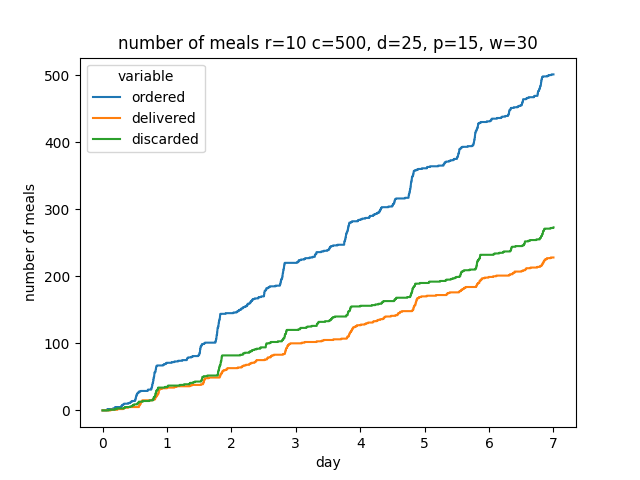
\includegraphics[width=\textwidth]{sections/run1/week_nd_1_food_ordering_distribution_500_10_25_30}
            \caption{example 1}
        \end{subfigure}
        \hfill
        \begin{subfigure}[m]{0.30\textwidth}
            \centering
            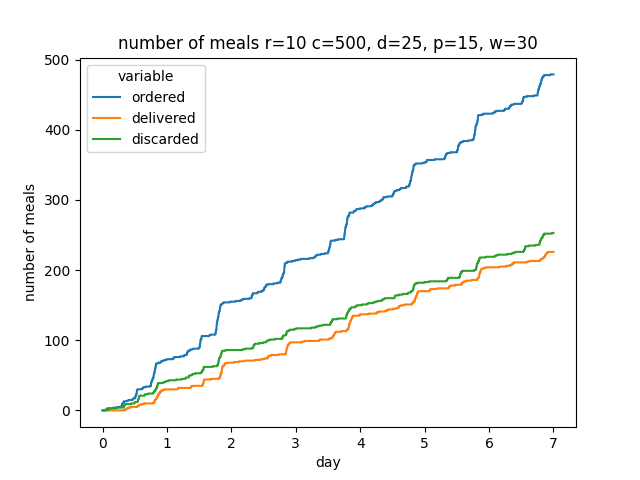
\includegraphics[width=\textwidth]{sections/run1/week_nd_2_food_ordering_distribution_500_10_25_30}
            \caption{example 2}
        \end{subfigure}
        \hfill
        \begin{subfigure}[m]{0.30\textwidth}
            \centering
            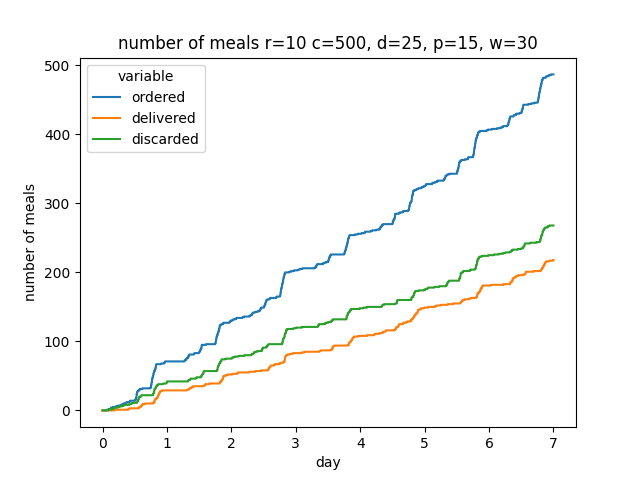
\includegraphics[width=\textwidth]{sections/run1/week_nd_3_food_ordering_distribution_500_10_25_30}
            \caption{example 3}
        \end{subfigure}
        \caption{Examples 25 deliverers}
        \label{fig:examples 25 deliverers}
    \end{figure*}
\end{center}
\begin{center}

    \begin{figure*}
        \centering
        \begin{subfigure}[m]{0.30\textwidth}
            \centering
            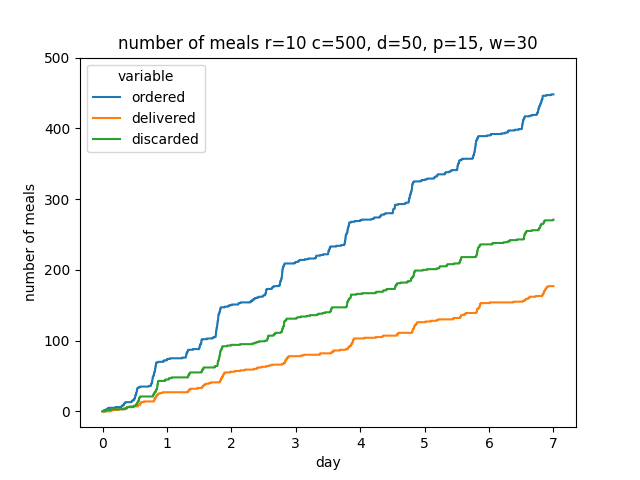
\includegraphics[width=\textwidth]{sections/run2/week_nd_1_food_ordering_distribution_500_10_50_30}
            \caption{example 1}
        \end{subfigure}
        \hfill
        \begin{subfigure}[m]{0.30\textwidth}
            \centering
            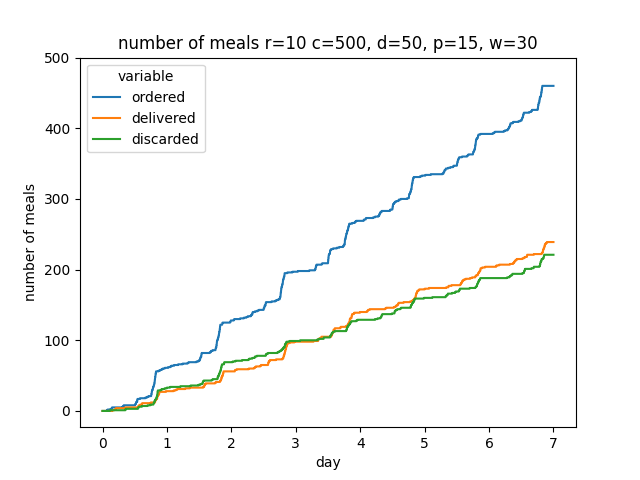
\includegraphics[width=\textwidth]{sections/run2/week_nd_2_food_ordering_distribution_500_10_50_30}
            \caption{example 2}
        \end{subfigure}
        \hfill
        \begin{subfigure}[m]{0.30\textwidth}
            \centering
            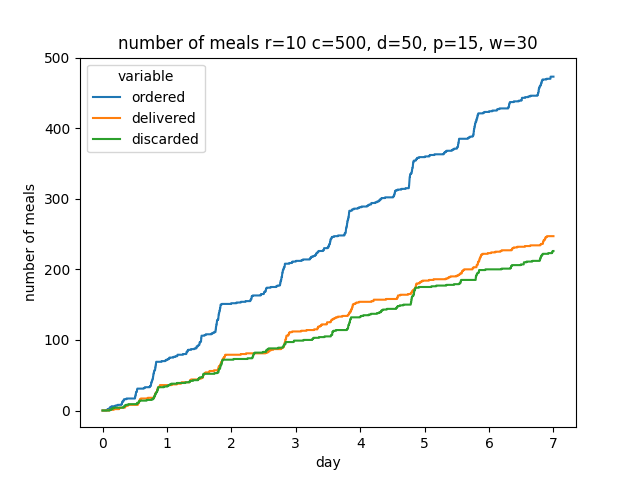
\includegraphics[width=\textwidth]{sections/run2/week_nd_3_food_ordering_distribution_500_10_50_30}
            \caption{example 3}
        \end{subfigure}
        \caption{Examples 50 deliverers}
        \label{fig:examples 50 deliverers}
    \end{figure*}
\end{center}

For the next run the delivery times were made longer.
The results are shown in figure~\ref{fig:examples 25 deliverers different wait time} and ~\ref{fig:examples 50 deliverers different wait time}
Now there is difference, the longer the allowed wait time the more meals are delivered and not discarded.

\begin{center}
    \begin{figure*}
        \centering
        \begin{subfigure}[m]{0.30\textwidth}
            \centering
            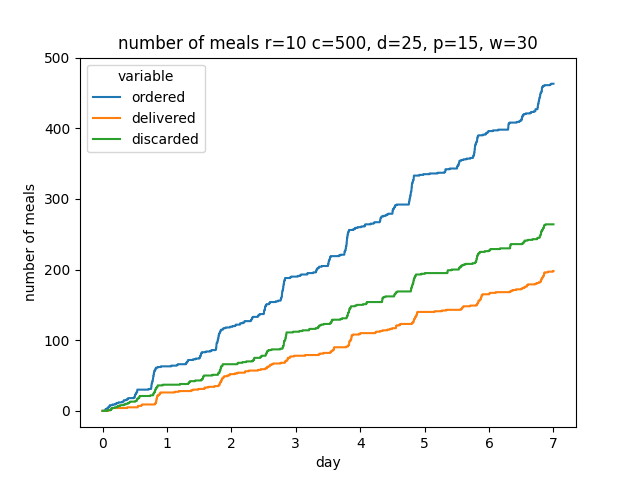
\includegraphics[width=\textwidth]{sections/run3/week_nd_1_food_ordering_distribution_500_10_25_30}
            \caption{30 min wait time}
        \end{subfigure}
        \hfill
        \begin{subfigure}[m]{0.30\textwidth}
            \centering
            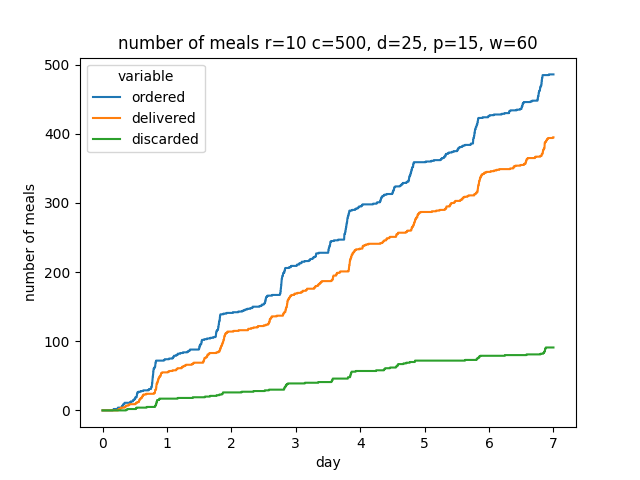
\includegraphics[width=\textwidth]{sections/run3/week_nd_2_food_ordering_distribution_500_10_25_60}
            \caption{60 min wait time}
        \end{subfigure}
        \hfill
        \begin{subfigure}[m]{0.30\textwidth}
            \centering
            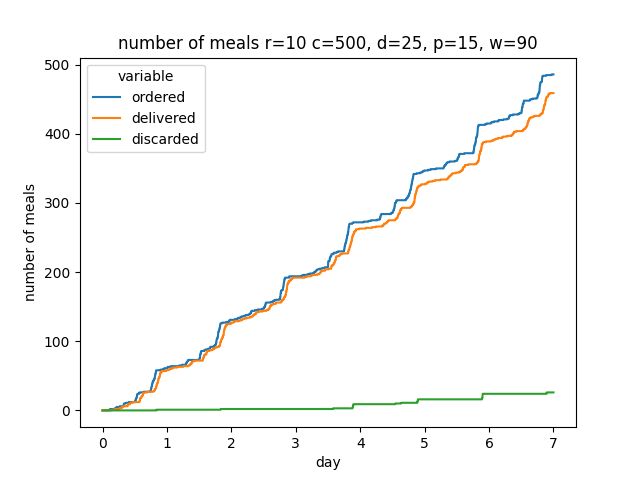
\includegraphics[width=\textwidth]{sections/run3/week_nd_3_food_ordering_distribution_500_10_25_90}
            \caption{90 min wait time}
        \end{subfigure}
        \caption{Examples 25 deliverers}
        \label{fig:examples 25 deliverers different wait time}
    \end{figure*}
\end{center}
\begin{center}

    \begin{figure*}
        \centering
        \begin{subfigure}[m]{0.30\textwidth}
            \centering
            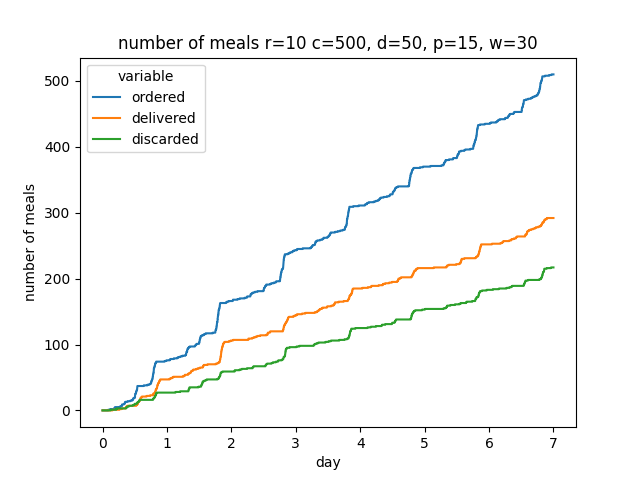
\includegraphics[width=\textwidth]{sections/run4/week_nd_1_food_ordering_distribution_500_10_50_30}
            \caption{30 min wait time}
        \end{subfigure}
        \hfill
        \begin{subfigure}[m]{0.30\textwidth}
            \centering
            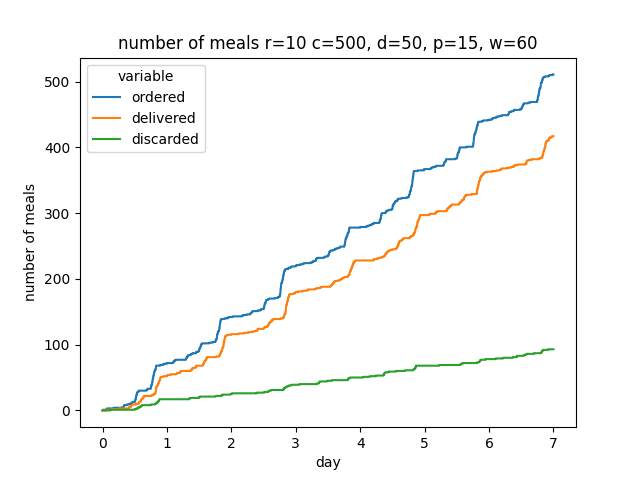
\includegraphics[width=\textwidth]{sections/run4/week_nd_2_food_ordering_distribution_500_10_50_60}
            \caption{60 min wait time}
        \end{subfigure}
        \hfill
        \begin{subfigure}[m]{0.30\textwidth}
            \centering
            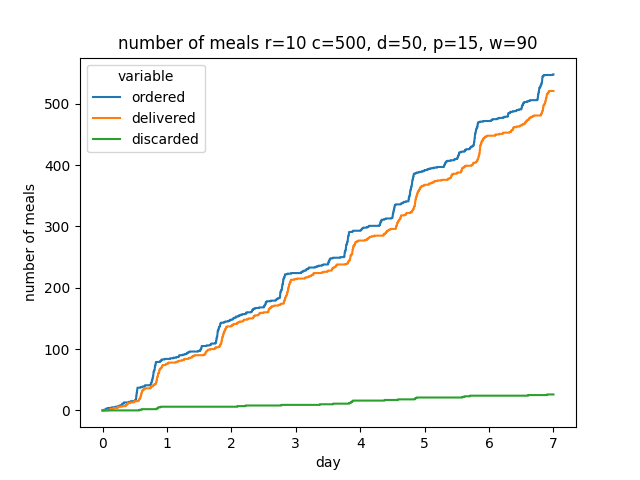
\includegraphics[width=\textwidth]{sections/run4/week_nd_3_food_ordering_distribution_500_10_50_90}
            \caption{90 min wait time}
        \end{subfigure}
        \caption{Examples 50 deliverers}
        \label{fig:examples 50 deliverers different wait time}
    \end{figure*}
\end{center}

We can tell from these results that the longer the waiting time the more deliveries are made,
Again there is not much difference between the number of deliverers.

To find out what the effect is of the number deliverers, the simulation was run for a waiting time of 60 and 90 minutes,
and 10 to 60 deliverers.
The result of these simulations, for a simulated week, are:

\begin{center}
    \begin{tabular}{ |c|c|c| }
        \hline
        waittime       & 60   & 90   \\
        nr. deliverers &      &      \\
        \hline
        \hline
        10             & 63\% & 69\% \\
        \hline
        20             & 75\% & 88\% \\
        \hline
        30             & 83\% & 96\% \\
        \hline
        40             & 87\% & 99\% \\
        \hline
        50             & 89\% & 97\% \\
        \hline
        60             & 80\% & 99\% \\
        \hline
    \end{tabular}
\end{center}

With this information the baseline is set.
A wait time of 90 minutes and 30 deliverers would be the best, more deliverers have the same result.

\subsection{Model variant 1}
The baseline is determined with the next settings:
\begin{center}
    \begin{tabular}{ |c|c|c| }
        \hline
        variable              & type & default \\
        \hline
        \hline
        number-of-restaurants & int  & 10      \\
        \hline
        number-of-customers   & int  & 500     \\
        \hline
        number-of-deliverers  & int  & 30      \\
        \hline
        prepair\_time\_mean   & int  & 15      \\
        \hline
        wait\_for\_deliverer  & int  & 90      \\
        \hline
    \end{tabular}
\end{center}

Now simulations will be run over a much longer period, also the number of delivered meals per deliverer is measured.

On 6 runs of simulated 10 weeks the results are:

\begin{center}
    \begin{tabular}{ |c|c|c|c| }
        \hline
        meals ordered & meals delivered & meals discarded & percentage delivered \\
        \hline
        \hline
        4857          & 4798           & 58             & 0.98                 \\
        \hline
        4839          & 4755           & 81             & 0.98                 \\
        \hline
        4958          & 4630           & 327             & 0.93                 \\
        \hline
        4773          & 4645           & 126             & 0.97                 \\
        \hline
        4895          & 4562           & 330             & 0.93                 \\
        \hline
        4800          & 4756           & 41             & 0.99                 \\
        \hline
        \hline
        4853          & 4691           & 160             & 0.96 \\
    \end{tabular}
\end{center}

A deliverer delivers per day  4691 / (10 * 7 * 24 + 60 * 30) = 3.9 meals


\subsection{Model variant 2}
For the second variant delivers may leave if they don't make enough money.
In the previous section a deliverer may have heard that a delivers can deliver 3.9 meals per day or 27.3 per week.

In this model if a deliverer delivers less then this number in a week they will stop delivering.


